\documentclass[12pt]{article}

\usepackage{amssymb,amsmath,amsfonts,eurosym,geometry,ulem,graphicx,caption,color,setspace,sectsty,comment,footmisc,caption,natbib,pdflscape,subfigure,array,hyperref,filecontents}
\normalem



\onehalfspacing
\newtheorem{theorem}{Theorem}
\newtheorem{corollary}[theorem]{Corollary}
\newtheorem{proposition}{Proposition}
\newenvironment{proof}[1][Proof]{\noindent\textbf{#1.} }{\ \rule{0.5em}{0.5em}}

\newtheorem{hyp}{Hypothesis}
\newtheorem{subhyp}{Hypothesis}[hyp]
\renewcommand{\thesubhyp}{\thehyp\alph{subhyp}}

\newcommand{\red}[1]{{\color{red} #1}}
\newcommand{\blue}[1]{{\color{blue} #1}}

\newcolumntype{L}[1]{>{\raggedright\let\newline\\arraybackslash\hspace{0pt}}m{#1}}
\newcolumntype{C}[1]{>{\centering\let\newline\\arraybackslash\hspace{0pt}}m{#1}}
\newcolumntype{R}[1]{>{\raggedleft\let\newline\\arraybackslash\hspace{0pt}}m{#1}}

\geometry{left=1.0in,right=1.0in,top=1.0in,bottom=1.0in}

\begin{document}

\title{The Spatial Uncertainty Problem:\\Characterization and Solutions Using Probability Distributions and SIMEX}
\author{The Dan Team}
\date{\today}
\maketitle

\setcounter{page}{0}
\thispagestyle{empty}

\doublespacing


\section{Introduction} \label{sec:introduction}

In studies of the effect of international development projects, the exact location of project implementation is often unknown, creating a source of uncertainty and difficulty in accurately ascribing effects to project implementation. Such spatial uncertainty may stem from insufficient project documentation. At AidData, when projects are geocoded, they are assigned a precision-code, which describes the resolution in land area at which we are certain about the location of a project. A precision code of 1 is used when the exact location is known. Values up to 8 are assigned when the available documentation can only provide information about a general location such as a district or even an entire country.
\\ \\
In the method presented, we describe a probability distribution for the implementation of projects in a region of interest in terms of dollars spent in the area using the information available at our resolution of spatial certainty and on the number of dollars allocated to each project. Further, we describe the use of this distribution to find an expected level of implementation. Finally, we demonstrate the use of linear regression modeling with measurement error with a modified version of SIMEX.

\section{Assumptions} \label{sec:assumptions}

With our method, we assume that the probability that any given dollar allocated to a project is spent within a region of interest is equal to the ratio of the area of overlap between the region of project allocation and the region of interest compared to the total area of the region of project allocation. For example, if the region of project allocation is an entire city, and the region of interest covers half the area of the city, the assumed probability that any given dollar is spent in the region of interest is one half. Our presumed region of project allocation is the area at the resolution of certainty for that project. Secondly, we assume independence of expenditure of separate dollars. Hence, the expenditure from a single project within a region of interest is assumed to be binomial distributed with parameters 

\begin{equation}
n = \mbox{dollars available to the project}
\end{equation}

and 

\begin{equation}
p = \frac{\mbox{area of overlap}}{\mbox{certain area of allocation}}
\end{equation}
\\ \\
Thirdly, the level of expenditure within a region of interest for different projects is assumed to be independent. Hence, the distribution for total expenditure from all known projects in a region of interest is assumed to be distributed as the sum of independent binomial distributed random variables.

\break

\section{Data} \label{sec:data}

Each project in a data set has a location, precision code, and dollar value associated with it. Based on the precision code, a geographic area is assigned to that project. For example, precision code 4 may be assigned to a district, precision code 7 a country. In figure 1, markers A1 and B1 indicate the latitudes and longitudes for two theoretical projects in Nepal called project A and B respectively. The geographic areas determined by the precision codes associated with projects A and B are indicated by markers A2 (a district) and B2 (the entire country) respectively.

\begin{figure}[!hbt]
\centering
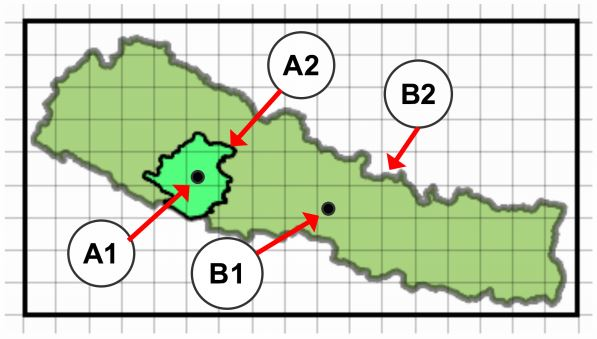
\includegraphics[width=0.3\textwidth]{reliability_map.JPG}
\caption{\label{fig:reliability_map}Project Areas}
\end{figure}

\break

\section{Calculating the Probability Distribution} \label{sec:distribution}

We calculate the distributions for money spent in the region of interest from project A and B
separately using parameters 

\begin{equation}
n_i = \mbox{dollars available to project \textit{i}}
\end{equation}

and

\begin{equation}
p_i = \frac{\mbox{area of overlap of ROI with project \textit{i}}}{\mbox{certain area of allocation for project \textit{i}}}
\end{equation}
\\
For example, we will calculate the distribution of expenditure in the area bounded by the large box in Figure 2:
\begin{figure}[!hbt]
\centering
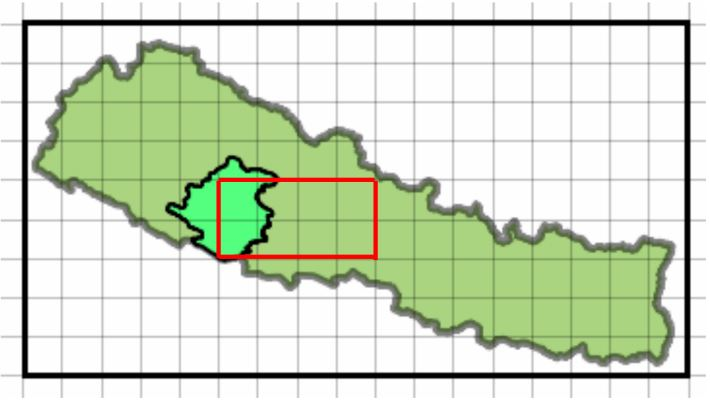
\includegraphics[width=0.3\textwidth]{region_of_interest.JPG}
\caption{\label{fig:region_of_interest}Region of Interest and Project Areas}
\end{figure}
\\ \\
We presume that project A covers approximately 4 cells with 2 cells of overlap and project B covers approximately 57 cells with 8 cells of overlap. We know that project A receives \$100,000 of aid and project B receives \$500,000 of aid. So,
\\$n_A = 100,000$
\\$n_B = 500,000$
\\$p_A = \frac{2}{4}$
\\$p_B = \frac{8}{57}$
\\Denote $A$,$B$ the number of dollars in region of interest from projects A and B, respectively. $A \sim \mbox{binom}(n_A,p_A)$ and $B \sim \mbox{binom}(n_B,p_B)$.
\begin{equation}
p(A=a) = \binom{100000}{a}\left(\frac{2}{4}\right)^a \left(1-\frac{2}{4}\right)^{100000-a}
\end{equation}

\begin{equation}
p(B=b) = \binom{500000}{b}\left(\frac{8}{57}\right)^b \left(1-\frac{8}{57}\right)^{500000-b}
\end{equation}

\noindent The probability density functions for $A$ and $B$:

\begin{figure}[!hbt]
\centering
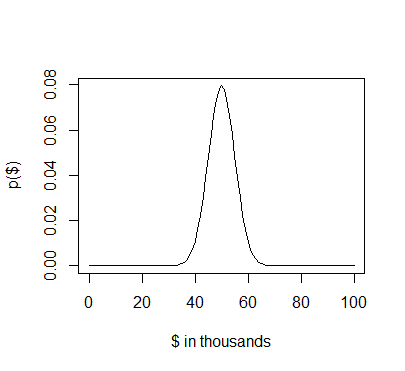
\includegraphics[width=0.3\textwidth]{dist_a.png}
\caption{\label{fig:dist_a}Probability Density of A}
\end{figure}

\begin{figure}[!hbt]
\centering
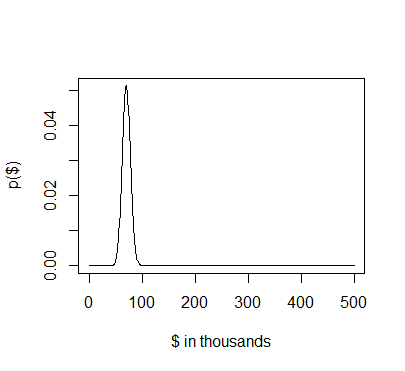
\includegraphics[width=0.3\textwidth]{dist_b.png}
\caption{\label{fig:dist_b}Probability Density of B}
\end{figure}

\break

\noindent Denote $S$ the sum of dollars from A and B spent in the region of interest. The distribution of $S$ can be calculated from the distributions of $A$ and $B$ using the formula\cite{butler1993distribution}: 
\begin{equation}
p(S = s) = \sum_{r=0}^{s}p(A=r) * p(B = s-r)
\end{equation}

\noindent The probability density function for $S$, with support $0$ to $100000+500000=600000$:

\begin{figure}[!hbt]
\centering
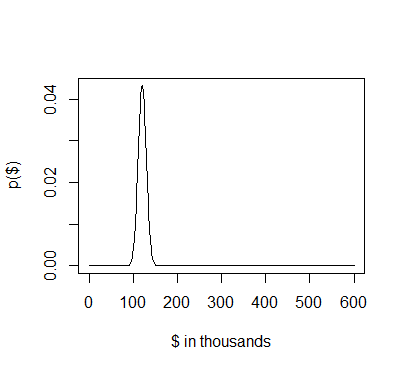
\includegraphics[width=0.3\textwidth]{dist_s.png}
\caption{\label{fig:dist_s}Probability Density of S}
\end{figure}


\noindent For the total expenditure in the region of interest we take the expected value of $S$:

\begin{equation}
E(S) = \sum_{s=0}^{600000}s*p(s) = 120,175
\end{equation}

\noindent We may also calculate the variance of $S$:
\begin{equation}
V(S) = \sum_{s=0}^{600000}(s-E(S))^2 * p(s) = 85,326
\end{equation}


\noindent In fact, we can calculate the distribution for the sum of expenditures in the region of interest from any number of projects by repeatedly applying a general version of the above formula.
\begin{equation}
p(Y + Z = j) = \sum_{i=0}^{j}p(Y=i) * p(Z = j-i)
\end{equation}
In this example we used $A$ and $B$ as $Y$ and $Z$, respectively to calculate $p(A + B = s)$. If we were to add a third project, C with expenditure in region of interest $C$, we could calculate the distribution of $S_{new}=A+B+C$ using $S$ as $Y$ in the above formula and $C$ as $Z$. The same could be done with a fourth and fifth project, ad infinitum, by repeatedly applying the general formula to the distribution of the sum and the additional project distribution.
\\ \\In practice, we do not use the number of dollars allocated to a project per se, but rather use units of \$10,000 for the sake of computational efficiency. Thus, we calculate the distribution of $A$ with $n_a = \frac{100000}{10000} = 10$. For maximum possible sum values in the millions of dollars this has no appreciable effect on the probability density function. The same principle can be applied with whatever unit is practical for the size of projects under consideration in terms of desired resolution of the probability density function and computational efficiency. In the example, units of \$1,000 were used in the actual calculation.

\break
\section{Linear Regression with Measurement Error in SIMEX} \label{sec:simex}
We demonstrate the use of our distribution of expenditure in a region of interest in a linear regression model with measurement error. In this model, we assume that a variable of interest, here population in an area, is causally, linearly related to aid funding in the region and elevation. As our measured value of aid funding, we use the expected value of the sum of expenditures from all projects overlapping a region in our data set. We assume that there is an appreciable level of error in our measurement, so we must use a modeling method that incorporates measurement error in addition to model error. One method that has been developed is SIMEX.
\\ \\
\noindent SIMEX (simulation and extrapolation method) is a method for incorporating measurement error of independent variables in regression analysis.\cite{shortIntro} SIMEX handles cases where the variance of the measurement error is constant (i.e., homoscedastic) or where the variance is non-constant (i.e., heteroskedastic), and handles a variety of estimators---including ordinary least squares and a host of generalized linear models, such as logit and probit. \\
\\
SIMEX treats the estimate of the beta coefficient as a function of measurement error. SIMEX simulates adding additional measurement error with increasing variance to the variable with error. It estimates new beta coefficients based on these new simulated data, and fits a function between the additional measurement error and the new beta coefficients. Using this function, it extrapolates the beta estimate to a point with no measurement error. \\\\
The simulation step is expressed in equation 11. $\lambda$ is a parameter that represents the amount of error being added to the original variable, where $\lambda$ is a set of monotonically increasing values (by default, SIMEX uses $\{\frac{1}{2}, 1, 1\frac{1}{2}, 2\}$). $X$ is the original data, and $X(\lambda)$ represents simulated data with additional error. $U$ represents a random amount of measurement error. 

\begin{equation}
X(\lambda)=X+\sqrt{\lambda}U
\end{equation}

Applications of SIMEX have used $U$ distributed as $N(0,\sigma_v^2)$, where $\sigma_v^2$ is the variance of the measurement error. However, we modify $U$ to be distributed according to an error distribution based on our sum distribution, where $U_s = S - E(S)$. This is easily conceptually justified as the difference between the actual value of $S$, the sum of expenditure in the region of interest, and $E(S)$, the expected value of $S$ used as our measure. Hence: 
\begin{equation}
X(\lambda)  = X + \sqrt{\lambda}(U_s) = X + \sqrt{\lambda}(S-E(S))
\end{equation}

\begin{figure}[!hbt]
\centering
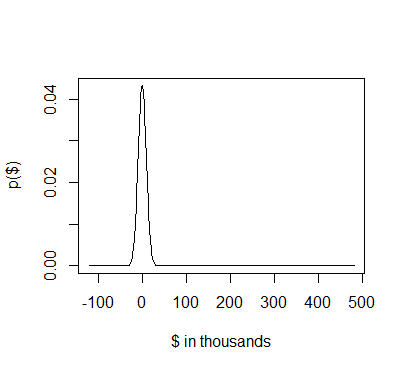
\includegraphics[width=0.3\textwidth]{dist_u.png}
\caption{\label{fig:dist_u}Distribution of Errors U in Thousands}
\end{figure}

[End section with full demonstration on data]

\break
\section{Conclusion} \label{sec:conclusion}

Our probabilistic method incorporates the spatial scale of projects and the spatial resolution of our certainty of location of project implementation. Using our method, we create a distribution for the level of project implementation in a region of interest, with which we can simulate the process of locating expenditure. The next steps are to validate the use of this probabilistic process through comparison with empirical distributions of expenditure and to develop methods allowing us to relax the assumptions of independence in expenditure.


\bibliographystyle{unsrt}
\bibliography{sum_binom}

\end{document}